%!TEX root = ../dissertation.tex
%\begin{savequote}[75mm]
%Nulla facilisi. In vel sem. Morbi id urna in diam dignissim feugiat. Proin molestie tortor eu velit. Aliquam erat volutpat. Nullam ultrices, diam tempus vulputate egestas, eros pede varius leo.
%\qauthor{Quoteauthor Lastname}
%\end{savequote}

\chapter{Holographic approach to arbitrary potential generation}

\section{Why do we need custom optical potentials?}
The main advantage of cold atoms experiments is an ability to prepare and probe the system on it's characteristic time and length scales (for a lattice models those would be a tunneling time and lattice spacing respectively). Quantum gas microscope enables us to observe our lattice system with a single site resolution, which lead to the first direct observation of superfluid to Mott insulator \cite{Bakr2010, bloch} as well as paramagnet to aniferromagent \cite{Simon2011, Parsons??} quantum phase transitions. However, in order to fully enable the capabilities of such quantum simulators one needs a tool to arbitrary control the shape of optical potentials in the system. This would enable preparation of desired initial states with high fidelity \cite{us, somebody else?}, studies of the systems with complex \cite{Tilman QPC, Roatti QPC} as well as dynamically changing \cite{??} geometries. To achieve this, one has to control the light intensity on a single lattice site scale, which can be achieved by means of spatial light modulators (SLM).

\section{Spatial light modulators in the image plane}
The first straight forward way is to use the microscope in reverse, by imaging a desired light pattern onto the atoms \cite{P. Schauß thesis, RMA thesis, MAZU thesis}. Although this method is very powerful for creating large scale, smooth-varying potentials, it has two major challenges. \textit{First}, the wavelength of conservative light potentials, that one wants to project, is generally very different from the atom imaging wavelength, which most quantum gas microscopes are optimized for. This can lead to significant distortion of the desired wavefront due to chromatic aberrations, if the imaging system is not specifically corrected for that. The first two leading orders of aberrations in this case are given by defocus and spherical aberration. This problem can be solved by either using an achromatic imaging system, that is wavelength insensitive in the desired range, or precompensating the imaged wavefront for the defocus caused by the imaging. \textit{Second}, it is fundamentally impossible to create $100 \%$ intensity modulation of the potential on the single site scale without using Fourier filtering and phase control of the wave front. 

To illustrate the last point, let's consider a single lens with a focal length $f$ and a fixed aperture of size $d$ in the Fourier plane (see fig~\ref{fig:DMD_lance}). To keep the math simple let's consider only two spatial dimensions $x$ and $z$. The sharpest feature that one can make in the image plane with constant phase wavefront in the Fourier plane is so called point spread function, with the resulting light intensity in the image plane given by $I(x) \sim sinc^2(\frac{\pi}{\Theta} x)$, where $\Theta = \frac{\lambda f}{d}$ (see fig~\ref{fig:DMD_lens} A). The question becomes: how can one make an intensity pattern that is periodic with period $\Theta$? Two different electric field profiles would give us the intensity profile that satisfies this requirement: $E_1 \sim \sqrt{(1+cos(\frac{\pi}{\Theta}x))/2}$ and $E_2 \sim cos(\frac{\pi}{2\Theta} x)$, both yielding $I \sim (1+cos(\frac{\pi}{\Theta}x))/2$ (see fig~\ref{fig:DMD_lens} B,C). The first one has only positive electric field components and hence the same phase, however it's Fourier transform requires the Fourier plane, that is double the size of our initial point spread function. The second one has the same Fourier plane size as the one we started with at the expense of having electric field oscillate between positive and negative values, or in other words the phase of adjacent maxima alternate between $0$ and $\pi$. This example shows us that using the phase control of the wave front allows us to increase the image plane resolution by a factor of two.
%The characteristic size of the feature is $FWHM = 0.84 \Theta$.

\begin{figure*}[t]
	\centering
	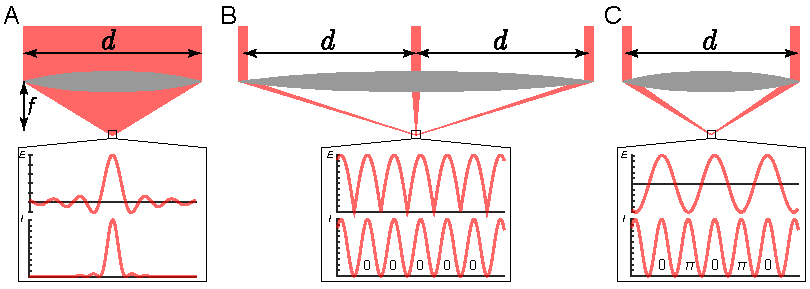
\includegraphics[scale=1]{figures/DMD_lance.pdf}
	\caption{{\bf Encoding phase and amplitude inforamtion with a grating}. {\bf A} When a light with initial wave vector $K_0$ passes through an amplitude grating with period $d$, it's outgoing wave vector can be changed by any integer multiple of grating wave vector $K_g\propto \frac{1}{d}$. {\bf B} Tow patches with the grating of the same period $d$ but different duty cycles $q_1$ and $q_2$ are shown. Since the duty cycle determines how much light goes through, the intensity of the outgoing light is proportional to the duty cycle. The outgoing light also carries the information about the local phase of the grating, by imprinting it onto the phase of outgoing electric field.}
	\label{fig:DMD_lance}
\end{figure*}

\section{Spatial light modulator in the Fourier plane}
Although, phase control of the electric field using image plane SLM can be achieved using number of phase coding methods along side with spatial filtering in the Fourier plane \cite{Lee1970, Goorden2014}, one still needs to correct for the aberrations, the beam encounters on its way form the SLM to the desired image plane (in our case we call it atom plane). Note, that one needs to correct for both intensity pattern, that eliminates the SLM, as well as any phase deviation from the desired wavefront, which might be particularly challenging for imaging systems with high numerical aperture, due to the breakdown of the paraxial approximation. In order to achieve the best possible quality of the optical potentials it would be desirable to be able to actively measure and compensate for aberration in the system, here the use of the SLM in the Fourier plane becomes particularly useful.

There are two main types of SLMs that are being used in such setups: liquid-crystal display (LED) based and digital micro-mirror device (DMD) based. LEDs can be configured to provide amplitude modulation or phase modulation of the incident beam, using the birefringence of liquid crystals. With optimization and feedback algorithms [83, 84], it is possible to create complex, re-programmable potentials, using this technology. However this type of SLMs have one major drawback when it comes to cold atoms experiments. Due to the nature of liquid crystals, they have to be placed into the switching electric filed, that oscillates with frequencies in $kHz$ range, causing the output light to blink at the same frequency. This blinking could potentially be a problem, since the typical trap frequencies of the atoms in optical lattice experiments lay in the same frequency range, and hence the blinking light might induce undesired heating in the system.

Another approach is to use a DMD, that consist of CMOS arrays of micromirrors on torsion hinges which can be switched
between two angles corresponding to the \textit{on} and \textit{off} directions. These devises are typically used in commercial video projectors, and are available with resolutions up to $2560 \times 1600$ pixels. The device used in our experiment is the Keynote Photonics FlexLight X3, which uses the Texas Instruments DLP 5500 chipset. The $1024 \times 768$ micromirror array has a pitch of $10.8 \mathrm{\mu m}$, micromirror tilts $\pm 12^{\circ}$ from normal, and an update rate of $5 \mathrm{kHz}$. The time required to switch between individual patterns is even shorter, on the order of a few $\mathrm{\mu s}$, which can allow dynamical control over the potential.

\section{Encoding phase information with DMD}
Since DMD does not have a build in ways to control the phase of the light field, one needs to find a way to encode this information using binary structure of the DMD pixels. In our experiment we use holographic approach that works as fallowing (see fig.~\ref{fig:DMD_grating}): Consider a plane wave incident onto an amplitude diffraction grating. The grating will crate multiple diffraction orders on the output, each satisfying the condition $k_n = k_0 + n*k_g$, where $k_n$, $k_0$ and $k_g$ are the wave vector of the n-th diffraction order, incident light and grating respectively. The grating wave vector is inversly proportional to the period of the grating $k_g \propto \frac{1}{d}$. We focus on the first diffraction order for the rest of the discussion. The overall spatial translation of the diffraction grating gets mapped onto the phase of the electric field in the diffracted order (see fig~\ref{fig:DMD_grating} B). Also the duty cycle of the grating will result in the intensity modulation of the out going light. Therefore by controlling the phase and duty cycle of the underlying grating we can locally control the phase and amplitude of the out going wave form the DMD \cite{Zupanchich thesis}.


\begin{figure*}[t]
	\centering
	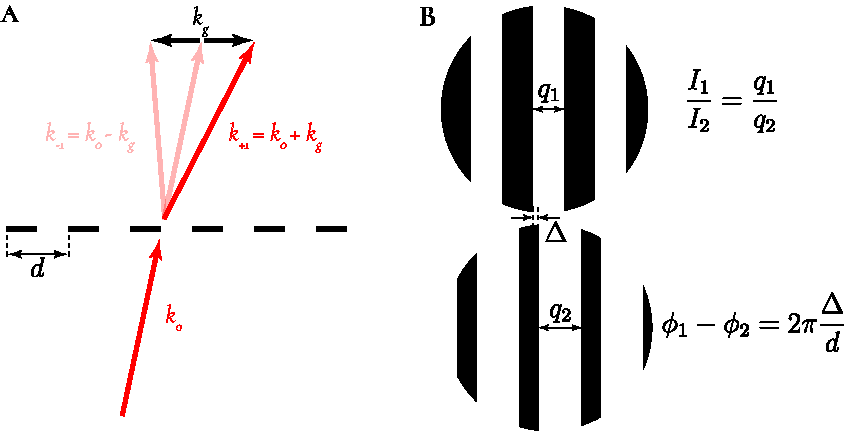
\includegraphics[scale=1]{figures/DMD_grating.pdf}
	\caption{{\bf Encoding phase and amplitude inforamtion with a grating}. {\bf A} When a light with initial wave vector $K_0$ passes through an amplitude grating with period $d$, it's outgoing wave vector can be changed by any integer multiple of grating wave vector $K_g\propto \frac{1}{d}$. {\bf B} Tow patches with the grating of the same period $d$ but different duty cycles $q_1$ and $q_2$ are shown. Since the duty cycle determines how much light goes through, the intensity of the outgoing light is proportional to the duty cycle. The outgoing light also carries the information about the local phase of the grating, by imprinting it onto the phase of outgoing electric field.}
	\label{fig:DMD_gratimg}
\end{figure*}

\section{Optical setup}
We chose to use the aperture of $500$ pixels (which approximately equals to $5.4 \mathrm{mm}$) in diameter on our DMD. In order to image it onto the objective Fourier plane, which is $18 mm$ in diameter we use the optical set up shown in the figure~\ref{fig:DMD_setup} A. In order to make the alignment easier and also to be able to control the image plane position of the potential without changing the hologram we use IP and FP mirrors (see fig.~\ref{fig:DMD_setup}). The FP mirror moves the beam primarily in the Fourier plane, since it's located very close to the image plane of the imaging system, and hence does not change the position of the beam in the image plane. The IP mirror position is chosen such that it primarily displaces the beam in the image plane. In order to understand the exact location of this mirror it is instructive to look at where the plane of the DMD (which is the Fourier plane of the overall imaging system with respect to the atoms) is imaged to (see fig~\ref{fig:DMD_setup} B). It is clear from the figure that this mirror is positioned exactly in the Fourier plane of the imaging system and hence moves the beam in the image plane.

Typically we use DMD to create potentials that have single site resolved features in one direction and slow varying amplitude in the other. The Fourier transform of such a pattern occupies entire Fourier plane along the direction of the narrow feature and only a small fraction along the other one, which is inversely proportional to the size of the slow varying amplitude. This implies that, if we would like to achieve the best power efficiency, we would like to match this profile with the intensity of the incoming beam. We accomplish this by having additional elliptical illumination channel with aspect ration $\frac{1}{7.5}$, along with the round illumination beam, primarily used for calibration purposes.

Since DMD and optical lattice don't have a common interferometric reference their relative position may drift in time. This means, that we need a way to track and stabilize their relative alignment. We do it by using the reflection of the both beams off of the superpolishid substrate and imaging them with separate camera in the intermediate image plane (see fig.~\ref{fig:DMD_setup}). This method provides us with the reference that almost coincides with the atom plane. We apply feedback using IP mirror of the DMD once every experimental cycle, corresponding to a frequency of $\sim 1 \mathrm{Hz}$. This allows us to stabilize the relative position to within $0.03$ lattice sites RMS. The residual noise is attributed to the air currents and mechanical vibrations of the breadboards.

\section{Calibration and aberration correction}
In order to achieve diffraction-limited resolution in the atom plane we need a way to map out the aberrations that occur on the optical path from DMD to the atom plane. The two main source of the phase error in our system are the curvature of the DMD chip, that is present due to the manufacturing process, and chromatic aberrations of the objective lance, that has $\sim 1 \frac{\mathrm{\mu m}}{\mathrm{nm}} $ of chromatic shift. We also need to compensate for the intensity profile of the beam that illuminates the DMD, in order to have spacial control over the amplitude of the electric field.

An aberration free lance bends a beam parallel to the optical axis, such that it passes through the focal point, and makes the phase of any such beam equal at that spot. If we take two beams in the Fourier plane they will interfere to create a periodic intensity modulation in the image plane, with the period inversely proportional to their spacing in the Fourier plane (see fig.~\ref{fig:DMD_cal_scheam}). The phase of this modulation is given by the relative phase between the beams, and the amplitude by the square root of the product of electric fields. Hence, by using one beam as a reference one can map out the relative phase and amplitude of any other beam by measuring the phase and amplitude of the resulting interference pattern \cite{Zupancic2016}.

First we preform theto calibration using a pinhole in the indeterminate image plane  detect the resulting intensity modulation (for more detailed description of this procedure see Master’s thesis by Philip Zupancic \cite{Zupancic thesis}). The size of the pinhole (in our case $10 \mathrm{\mu m}$) is chosen such, that it is much smaller then the smallest period of the intensity modulation, created by interfering two beams from the opposite ends of the Fourier plane. We use patches with diameter $\sim \frac{1}{15}$ of the full Fourier plane to create local beams from the previous example. This procedure is relatively fast and has high signal to noise ration, resulting in typical wave front flatness of $\sim \frac{\lambda}{40}$. By using a single reference patch we are also able to create the amplitude map of the illumination beam \cite{Zupancic2016}.  

Next we create the phase map from the intermediate plane to the atom plane, using atoms as a detector. We use weekly interacting BEC of $\sim 400$ atoms in the harmonic trap with a diameter of $\sim 30$ lattice sites to read off the phase of the interference pattern. The intensity profile results in the density modulation of the atomic cloud due to the Stark shift exerted onto the atoms by the light (see fig.~\ref{fig:DMD_FPcal}). This technique has a number of limitations: since we rely on atoms to map out the resulting intensity pattern, we require at least few oscillations of the potential within our cloud size. This limits our ability to measure the potential with large spacing, or form the Fourier point of view the patches that are close together. On the other hand the patches that are nearly entire Fourier plane apart are also challenging to measure, since they result in the intensity modulation with a period of $\sim 1$ lattice site. Hence using the same technique with a fixed reference patch, as was used in the intermediate plane, does not seem feasible. It is also challenging to acquire enough statistic in order to properly map out the intensity of the resulting potential, so the creation of the amplitude map is not feasible either. Here one should note that the amplitude map should stay unchanged form the intermediate plane one, since there is no spatial dependence of the transmission of the optical elements in between two planes. Hence it is sufficient to use the amplitude calibration from the intermediate image plane all the way to the atom plane.

In order to overcome the above limitations, instead of keeping one patch as a reference we keep the spacing between two patches fixed and then scan  this pair across the Fourier plane (see fig.~\ref{fig:DMD_FPcal}). The spacing  is chosen such that the resulting intensity modulation has a period of $\sim 4$ lattice sites. We average the resulting atom density distribution over up to $7$ realizations for a given pair of patches, allowing us to fit $\sim 7$ periods of modulation. Combined with the precise control over the relative stability of the DMD pattern with respect to the lattice, provided by the tracking, allows us to achieve $66\%$ confidence interval for phase estimation of $0.27 \mathrm{rad}$ or $\sim \frac{\lambda}{23}$. 

Since we only measure the difference between a pair of patches, we effectively measure the derivative of the phase profile with this method. We reconstruct the phase by using a polynomial fit up to $7\mathrm{th}$ order. This procedure give us a phase profile of the wavefront along one line. In order to reconstruct the full $2\mathrm{D}$ map we repeat this process along 6 different cuts though the Fourier plane, and then use a smooth surface parametrized by the Zernike polynomials up the $6\mathrm{th}$ order to fit the full $2\mathrm{D}$ surface. Since in the typical experimental setting we only use a small part of the Fourier plane for our patterns, after applying the full $2\mathrm{D}$ phase correction according to the reconstructed phase front, we repeat the calibration along the line through the center of the pattern region. The above procedure results in RMS error of the phase better then $\frac{\lambda}{14}$ across the whole Fourier plane.

\section{Holographic potentials and their limits}
To create a desired potential on the atoms we rely on the imaging system property, that electric field in the image plane equals to the Fourier transform of the field in the Fourier plan. Therefore in order to create desired potential we first numerically find it's Fourier transform (note that in general it will be a complex valued function),then in order to represent both amplitude and phase information of the desired potential we use the grating method, that encodes them in local phase and duty cycle of the grating respectively (see fig.~\ref{fig:DMD_hologram}). As long as we know the aberration profile in our system we can easily correct for it by locally modifying the phase to $\phi_{total} = \phi_{target} - \phi_{aberrations}$ and amplitude $A_{total} = \frac{A_{target}}{A_{beam}}$.

If our DMD had pixels with a gray scale, the potential would be limited by the discretization of individual pixels, however the binary nature of the device create an additional noise source that limits the precision of the resulting potentials. One straight forward way to binarize the hologram is to switch pixel with index $(i,j)$ \textit{on} if 
\begin{equation}
\left| k_x i + k_y j + \phi_{total} \; mod \: 2 \pi \right| < arcsin(A_{total}),
\end{equation}
and \textit{off} otherwise. Here $k_x$ and $k_y$ are $x$ and $y$ components of an a priory chosen wave vectors of the underlying grating. Such method has one straightforward problem, when one of the components of the grating wave vector is zero. In this case the stripes of the grating exactly coincide with pixels of the hologram, and if the wave vector is not equal to a integer number of pixels, result in the distortion of the desired potential (see fig.~\ref{fig:DMD_K_rotation} A). This problem can be avoided by slightly randomizing the pixels at the edge of the slit, using the function 
\begin{equation}
\frac{1}{2}(tanh((p(i,j) + arcsin(A_{total}))/\xi) - tanh((p(i,j) - arcsin(A_{total}))/\xi)),
\end{equation}
where $p(i,j))=\left| k_x i + k_y j + \phi_{total} \; mod \: 2 \pi \right|$ and $\xi$ is a parameter that control the "smoothness" of the distribution (see fig.~\ref{fig:DMD_K_rotation} B). Now we compare if the value of this function at any pixel position is grater then a randomly chosen number between $0$ and $1$, we set pixel \textit{on} and \textit{off} otherwise. From figure~\ref{fig:DMD_K_rotation} A it is clear that this method helps to reduce the effect of "bad" grating alignments, however it comes at a cost of increasing overall noise on the potential. This is easy to understand, since the more random we make the potential, the more likely it is to flip otherwise correct pixel value. It fallows form the discussion above, that in order to archive the best performance with the holograms it is beneficial to use nearly deterministic method of binarization away from "bad" angles. 
 
Another parameter that could effect the hologram quality is the absolute value of the grating wave vector, or in simple terms a period of stripes. Although one might expect to find some optimal value for this parameter, our numerical simulations show, that the quality of the resulting potential stays unaffected in a wide range of parameters (see fig.~\ref{fig:DMD_K_vary}A). Surprisingly, even when the stripe width becomes very small and additional grating emerges with separate wave vector (see fig.~\ref{fig:DMD_K_vary}B) the image is not being effected too much. Additionally the unwanted stuff in the image plane can be easily removed by spatial filtering.
 
We also try to determine the optimal value of the parameter $\xi$. To do that, we take the difference between two cuts, that are separated by one lattice site, through the resulting image plane profile. The introduction of the random parameter makes the resulting image plane profile to vary slightly from realization to realization. Therefore one can ask the question, what is the probability to obtain a pattern with desired maximum difference between two cuts? Our numerical results (see fig.~\ref{fig:DMD_rand_vary}) suggest that introduction of a small amount of randomness can lead to the improved results compared to the strictly deterministic case. Although, more complex way to reduce the binazization artifacts like error diffusion algorithms \cite{floyd, Hu2018} have been studied, their application in our system does not improve the results. 

